\chapter{Uitwerking}
{\samenvatting Deze masterproef maakt een monitoringsservice met een bijhorende monitoringsAPI die de monitoringsinformatie beschikbaar stelt. De API zal de resultaten bijhouden in een databank deze databank bevat de configuratie gegevens, de resultaten en de beschrijvingen van de verschillende testen. De API doorloopt voor elke aanvraag een opeenvolging van stappen. Zo wordt eerst de aanvraag geparset, vervolgens wordt een query gemaakt en uitgevoerd. Het resultaat van deze query wordt omgevormd tot objecten die vervolgens ge\"encodeerd worden. De website zal deze ge\"encodeerde objecten eerste decoderen en vervolgens visualiseren. Het laatste project is de monitoringsservice deze zal via de API de testen binnenhalen. Deze worden vervolgens uitgevoerd en het resultaat wordt teruggestuurd naar de API.}
\section{Databank}
\npar
De databank bestaat uit meerdere tabellen die met elkaar verbonden zijn:
\begin{enumerate}
\item users, deze tabel houdt info bij over de login gegevens die gebruikt worden.
\item testbeds, deze tabel houdt info bij over de testbeds die gemonitord worden.
\item testDefinitions, deze tabel bevat beschrijvingen van de verschillende testen.
\item parameterDefinitions, deze tabel bevat per rij een beschrijving van een parameter.
\item returnDefinitions, deze tabel bevat een beschrijving van de waarden die teruggegeven worden. 
\clearpage
\item testInstance, deze tabel bevat een object van een testDefinitie.
\item parameterInstance, de waardes van de parameters.
\item results, de resultaten
\item subResults, de tussen resultaten.
\end{enumerate}
\npar
Dit alles is geschetst in Figuur \ref{structDatabase} op volgende pagina. Hier zijn de tabellen gegroepeerd op basis van functionaliteit om een beter overzicht te behouden.
\mijnfiguur{width=1\textwidth}{structDatabase}{De stuctuur van de databank}
\clearpage
\subsection{Definities}
\npar
De eerste groep tabellen bevat de definities. De databank is zelf-documenterend. De definities bevatten een omschrijving van een test. Hierbij worden de parameters en tussenresultaten ook opgeslagen. Deze worden opgenomen in een extra tabel om meer flexibiliteit toe te laten. Door de parameters en tussen resultaten in een andere tabel onder te brengen, is het mogelijk om verschillende testen met een variabel aantal tussenresultaten en parameters op te slaan.
\subsection{Instanties}
\npar
Deze tabel houdt de instanties bij. Een testinstantie is de test zelf. Als de vergelijking met object-geori\"enteerd programmeren gemaakt wordt, dan is een testDefinitie een klasse zelf en de instance is dan een object. Deze opsplitsing heeft het voordeel dat de beschrijving van een test apart opgeslagen kan worden. Het is vervolgens zeer eenvoudig om meerdere instanties aan te maken. Ook laat systeem de nodige flexibiliteit om de nieuwe definities aan te maken. Net zoals bij de definities zijn de ingevulde waarden hier ook ondergebracht in een aparte tabel. Dit is met dezelfde reden, namelijk het toelaten van een variabel aantal parameters.
\subsection{Configuratie gegevens}
\npar
De configuratie gegevens bestaan uit de gebruikers en testbeds. De gebruikers zijn belangrijk omdat ze de login informatie bevatten die gebruikt worden door de automated tester om testen uit te voeren. Zo zal een login test een gebruiker nodig hebben die de juiste rechten heeft op dat testbed.
Naast de gebruikers is er ook de informatie over de testbeds. De testbeds hebben o.a. elke een eigen url, urn en naam. Deze informatie wordt in deze tabel ondergebracht. Zowel een gebruiker als een testbed kan/kunnen vervolgens opgegeven worden als een parameter van een testinstance. 
\subsection{Resultaten}
\npar
Deze tabel zal alle resultaten bijhouden. Elk resultaat heeft een bijhorende logfile, deze wordt momenteel niet opgeslagen in de databank, maar apart op harde schijf. Het pad naar de logfile wordt vervolgens opgenomen in de databank. Dit heeft als voordeel dat de databank niet overvol geraakt met logfiles. Op die manier kunnen bijvoorbeeld alle tussenresultaten 6 maanden bijgehouden worden terwijl de logfiles maar voor 2 maanden bijgehouden worden.
\clearpage
\section{Webservice / API}
\npar
De webservice zal informatie uit de databank ophalen en omvormen naar object. Dit verloopt in een aantal fasen, zoals schematisch weergegeven in Figuur \ref{structAPI}.
\mijnfiguur{width=1\textwidth}{structAPI}{De werking van de API}
\clearpage
\subsection{Fasen}
\npar
De stappen die overlopen worden zijn:
\begin{enumerate}
\item parsen aanvraag.
\item query opbouwen
\item uitvoeren query
\item opbjecten bouwen
\item encoderen objecten
\end{enumerate}
De tekst hieronder zal kort een overzicht geven van elke stap. Op het einde van de uitleg wordt 
\subsection{Parsen aanvraag}
\npar
Er zijn drie soorten aanvragen, de eerste gaat om het opvragen van configuratie gegevens, terwijl de volgende ophalen en toevoegen van resultaten bevat. De laatste groep aanvragen heeft te maken met het toevoegen van resultaten en bijhouden van de scheduling.
\npar
Aanvragen van de eerste groep zijn:
\begin{enumerate}
\item testbed, geeft informatie weer over een of meerdere testbeds.
\item user: geeft informatie weer over een of meerdere users.
\item testDefinition: geeft informatie weer over de opbouw van een test.
\item testInstance: geeft informatie weer over de testen.
\end{enumerate}
De tweede groep gaat over het opvragen van resultaten:
\begin{enumerate}
\item last: geeft de laatste resultaten weer.
\item list: geeft een lijst met resultaten weer.
\item q: wordt gebruikt voor het afhandelen van GENI aanvragen. Hierbij wordt de aanvraag zelf ge\"encodeerd in json. Het antwoord wordt vervolgens ge\"encodeerd volgens de GENI dataschema's.
\end{enumerate}

\clearpage
Een derde groep aanvragen verzorgt het uitvoeren van de testen en de scheduling:
\begin{enumerate}
\item testInstance gefilterd op nextrun: geeft de testen weer die uitgevoerd moeten worden op een zeker tijdsstip.
\item updateNextrun: zal het moment waarop de volgende test uitgevoerd moet worden aanpassen.
\item addResult: zal een nieuw resultaat toevoegen aan de databank hiervoor met het type wel een HTTP-post request zijn.
\end{enumerate}
Voor een complete lijst van aanvragen en filter mogelijkheden wordt verwezen naar de bijlage.
\subsection{Aanmaken query}
\npar 
In deze stap wordt de query aangemaakt; de filters die opgegeven werden bij de parameters worden vertaald naar SQL syntacs. Bijvoorbeeld:
\begin{lt}
/last?testdefinitionname=ping,stitching
\end{lt}
zal vertaald worden naar een where clause :
\begin{lt}
... where testdefinitionname IN (ping,stitching) ...
\end{lt}
\npar
Dit gebeurd in de QueryBuilder, een interface die overge\"erfd wordt zodat het mogelijk is om de aanvragen op verschillende manieren te doen. De GENI aanvraag zal bijvoorbeeld door aan andere queryBuilder afgehandeld worden dan een standaard aanvraag.
\subsection{Uitvoeren query}
\npar
Deze stap is het uitvoeren van de query op de databank hiervoor wordt de php-pgsql module gebruikt die ervoor zorgt dat PHP verbinding maken met een postgreSQL databank.
\clearpage
\subsection{Bouwen objecten}
\npar
In deze stap worden het resultaat van de query lijn per lijn overlopen en worden objecten gevormd. Door de structuur van de databank worden meerdere lijnen samengenomen om een object te vormen. Dit komt door de aparte tabellen die gelinkt worden, waardoor er voor elke parameter een andere lijn ontstaat.
\npar
Om compabiliteit te verhogen worden er geen klassen zoals testbed en user aangemaakt, maar wordt alles direct opgeslagen in geneste array. Merk op dat in PHP arrays zowel een map als een array is. Hierdoor gaat er minder tijd verloren met de aanmaak van objecten om vervolgens de gegevens terug om te vormen naar het specifieke dataschema. Dit wordt gedaan in de Fetcher, opnieuw wordt hier gebruik gemaakt van overerving om andere structuren zoals voor GENI datastore te voorzien.
\subsection{Encoderen van objecten}
\npar
Dit is de laatste stuk in het process die voor de encodering zorgt. De encodering maakt het mogelijk om objecten te versturen over een netwerk. De encodering wordt gedaan in JSON door de formatter. Door overerving kan hier gemakkelijk gezorgd worden voor bijvoorbeeld xml-encodering.
\section{Service}
\npar
De service werkt met meerdere threads, er is een hoofdthread die testen ophaalt via de API. Vervolgens zal deze thread de testen toevoegen aan een queue. Een threadpool zal de testen een voor een uit de queue halen en uitvoeren. De grootte van de testpool wordt meegegeven bij het opstarten van het programma, standaard is dit het aantal cpu cores * 2 +1.
\npar
Elke test draait op een aparte thread. Tijdens het uitvoeren van een test wordt er verbinding gemaakt met een over meerdere testbeds. Dit gebeurt via de jFed automated tester module, een onderdeel van jFed. Deze geeft een xml file terug waar de tussenresultaten uit geparset worden. Deze resultaten worden vervolgens doorgegeven aan de resultuploader.
\npar
De resultuploader is een aparte thread die resultaten doorstuurt naar de API. Hierbij wordt ook de volgende uitvoeringstijd aangepast. Dit proces wordt beschreven in Figuur \ref{structService}.
\mijnfiguur{width=1\textwidth}{structService}{De werking van de monitoringsservice}
\clearpage
\section{Website}
\npar
De website bestaat uit een aantal verschillende interface. De eerste is de FLS (First Level Support) monitor deze heeft het doel de status van de testbeds zeer eenvoudig weer te geven. Een screenshot is te zien in Figuur \ref{FLSnieuw}.
\mijnfiguur{width=1\textwidth}{FLSnieuw}{FLS monitor}
\npar
Een volgende view wordt gebruikt om detail resultaten weer te geven van een type testen. In Figuur \ref{loginnieuw} wordt een overzicht gegeven van de login testen\footnote{Login2 in de titel is te verklaren dat dit login testen zijn voor aggregate manager 2}. Op deze figuur kan eenvoudig afgelezen worden dat de test voor het eerste testbed mislukt is, stap twee en vier (in rood) zijn mislukt. Diezelfde test is wel gelukt voor wall1 en wall2, maar met een waarschuwing voor stap 5.
\mijnfiguur{width=1\textwidth}{loginnieuw}{Overzicht van resultaten van de login testen.}
\clearpage
\npar
Tenslotte is er nog een overzicht van de geschiedenis van een specifieke test, dit is zichtbaar in Figuur{histnieuw}. Wanneer de cursor over een tussenresultaat gaat, verschijnt er een tooltip\footnote{Maakt gebruik van powertip, beschikbaar op http://stevenbenner.github.io/jquery-powertip/} waarop de naam van de subtest samen met de status wordt weergegeven\footnote{Dit is ook mogelijk bij de weergave van een test.}.
\mijnfiguur{width=1\textwidth}{histnieuw}{Geschiedenis van een login test.}
\npar 
Bij elke test is het mogelijk om de console uitvoer te bekijken, deze is beschikbaar in de log.
\begin{figure}[H]
\centering
\begin{subfigure}{.45\textwidth}
  \centering
  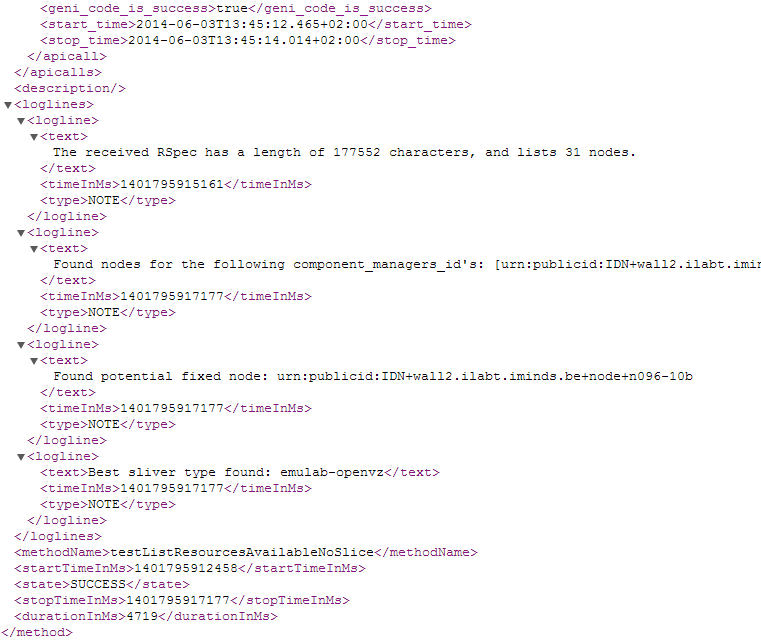
\includegraphics[width=.9\textwidth]{overviewxml}
  \caption{De originele overview in XML formaat}
\end{subfigure}
\begin{subfigure}{.45\textwidth}
  \centering
  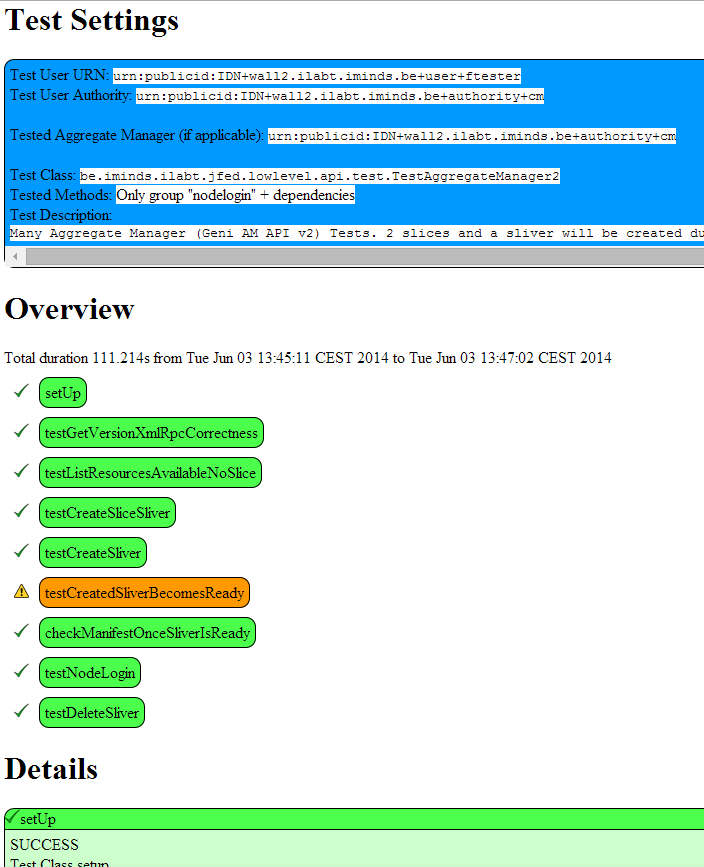
\includegraphics[width=.9\textwidth]{overviewhtml}
  \caption{Overview in html formaat}
\end{subfigure}
\caption{Naast de console uitvoer zijn ook het originele resultaat in XML formaat en het overeenkomstige HTML formaat beschikbaar.}
\end{figure}
